\documentclass{standalone}

\usepackage{amsmath,amsfonts,amssymb,amsthm,mathtools} 
\usepackage{fontspec}            % пакет для подгрузки шрифтов
\setmainfont{Burst My Bubble}   % задаёт основной шрифт документа

% why do we need \newfontfamily:
% http://tex.stackexchange.com/questions/91507/
\newfontfamily{\cyrillicfonttt}{Burst My Bubble}
\newfontfamily{\cyrillicfont}{Burst My Bubble}
\newfontfamily{\cyrillicfontsf}{Burst My Bubble}
% Иногда тех не видит структуры шрифтов. Эти трое бравых парней спасают ситуацию и доопределяют те куски, которые Тех не увидел.

\usepackage{unicode-math}     % пакет для установки математического шрифта
\setmathfont{Asana Math}      % шрифт для математики

\usepackage{polyglossia}      % Пакет, который позволяет подгружать русские буквы
\setdefaultlanguage{russian}  % Основной язык документа
\setotherlanguage{english}    % Второстепенный язык документа

\usepackage{pgf,tikz,pgfplots}
\usetikzlibrary{arrows,calc}
\usepackage{relsize} 

\usepackage{graphicx} 
\usepackage{rotating}
\usepackage{xcolor}
\usepackage{color}

%\newcommand{\Big}{\fontsize{50}{60}\selectfont Foo}

\definecolor{lmcolor}{HTML}{1B4c63}


\begin{document}

\centering

\begin{tikzpicture}[scale=1,decoration={random steps,segment length=1mm,amplitude=0.2pt}]

% Radius of regular polygons
\begin{scope}[rotate=30]
  \newdimen\R
  \R=6.4cm
  \coordinate (center) at (2,2);
 \draw (0:\R)
     \foreach \x in {60,120,...,360} {  -- (\x:\R) }
              -- cycle (300:\R)
              -- cycle (240:\R)
              -- cycle (180:\R)
              -- cycle (120:\R)
              -- cycle (60:\R)
              -- cycle (0:\R) [line width=1.9mm,color=lmcolor,fill=white,fill opacity=0.1];
\end{scope}

\begin{scope}[xshift=-4cm,yshift=-3.5cm,scale=0.9]
% picture with money
\node[inner sep=0pt] (russell) at (5.6,4.7){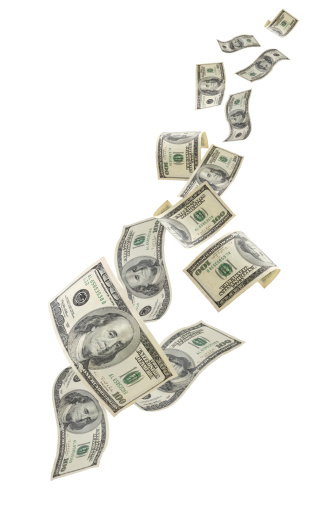
\includegraphics[angle=-190,scale=0.165]{mmm.jpg}};

%axis
\pgfplotsset{every axis/.append style={line width=1pt}}
\begin{axis}[%
axis x line=middle,  xlabel=$Y$,
axis y line=middle,  ylabel=$r$,
label style = {at={(ticklabel cs:1.1)}},
xmin=0,   xmax=6.99,
ymin=0,   ymax=7,
xticklabels={},
yticklabels={},
every inner x axis line/.append style={->},
every inner y axis line/.append style={->},
decoration={random steps,segment length=5pt,amplitude=0.3pt},decorate,
every tick/.style={thick,black,decorate}
]
\begin{scope}[decoration={random steps,segment length=3pt,amplitude=0.5pt},decorate]
%Shift IS-LM
\addplot [red, samples=30, domain=1.25:6.4] {8/x} node[right] {$IS$};
\addplot [lmcolor, samples=30, domain=1:6] {1.5^(x-2)} node[right] {$LM'$}; 
\addplot [lmcolor, samples=30, domain=0.7:4.7] {1.5^(x - 1) + 1} node[above] {$LM$}; 
\end{scope}
\end{axis}
%arrows between intersections
\draw[->,very thick, black, >=stealth'] (3.6,3.25)--(4.6,2.5) node[sloped,above, midway] {\footnotesize $\mathsmaller{\Delta M>0}$};
\end{scope}
%caption
\draw[color=black] (-4.2,3.2) node[right,scale=1.65] {{\color{lmcolor} {\fontspec{Comic Sans MS}{LM крутится - лавэха мутится!} }}};

\end{tikzpicture}

\end{document}


























































